\chapter{RESULTADOS E DISCUSS\~AO}
\label{cap:capitulo4}

\section{Desempenho dos modelos}
%Apresentar e comparar os resultados dos diferentes modelos utilizados.

Os resultados obtidos pelos modelos apresentaram variações significativas em termos de precisão, tanto nas previsões pontuais quanto nos intervalos de confiança, refletindo diferentes graus de precisão para cada cenário analisado. A análise dos resíduos revelou-se particularmente interessante, pois evidenciou comportamentos distintos em função da sazonalidade, com variações marcantes observadas em diferentes períodos do ano.

\subsection{Rio Jequitinhonha}

Iniciando pela menor bacia hidrográfica estudada, os resultados revelaram-se bastante satisfatórios, especialmente no que se refere ao modelo de Regressão Linear, que se destacou com previsões precisas, tanto em termos pontuais quanto nos intervalos de confiança. Este modelo demonstrou uma capacidade robusta de capturar a dinâmica hidrológica do rio, refletindo precisão nas métricas e desempenho consistente, aliado a um tempo de execução significativamente reduzido. Em contrapartida, o modelo (simples) SeasonalNaive apresentou resultados abaixo das expectativas em todas as situações avaliadas. (figura \ref{fig:jequiti_SN_WFV})

Com um MAPE extremamente elevado, de 150\%, os resultados indicaram um viés significativo de superestimação, conforme evidenciado pela métrica PBIAS. Verificando a KGE, ficou negativa. Em outras palavras, isso significa que o modelo não apenas falha em capturar a variabilidade dos dados observados, mas também introduz erros que o tornam menos eficaz do que uma abordagem simplista, como prever a média histórica. Embora a análise superficial da qualidade dos intervalos de confiança pudesse sugerir um desempenho satisfatório do modelo, uma inspeção mais detalhada revela uma incongruência: os valores inferiores do intervalo (lo-95) foram calculados abaixo de zero, o que não faz sentido para o rio em questão, pois implicaria na ausência total de vazão, algo inviável para as condições medidas pela estação. Além disso, o atraso (\textit{delay}) da série prevista foi considerável, atingindo 56,88 dias, com um desvio-padrão de 61,3 dias, sugerindo que um evento pode demorar mais de 60 dias para ser refletido na previsão do modelo.

Considerando o desempenho insatisfatório do modelo SN, a análise foi encerrada neste ponto, sem proceder com a avaliação dos resíduos ou a análise da importância das variáveis. O modelo foi incluído apenas para fins comparativos. A análise mais aprofundada será dedicada aos modelos mais complexos, que apresentaram desempenho superior.

\begin{figure}[!h]
	\centering
	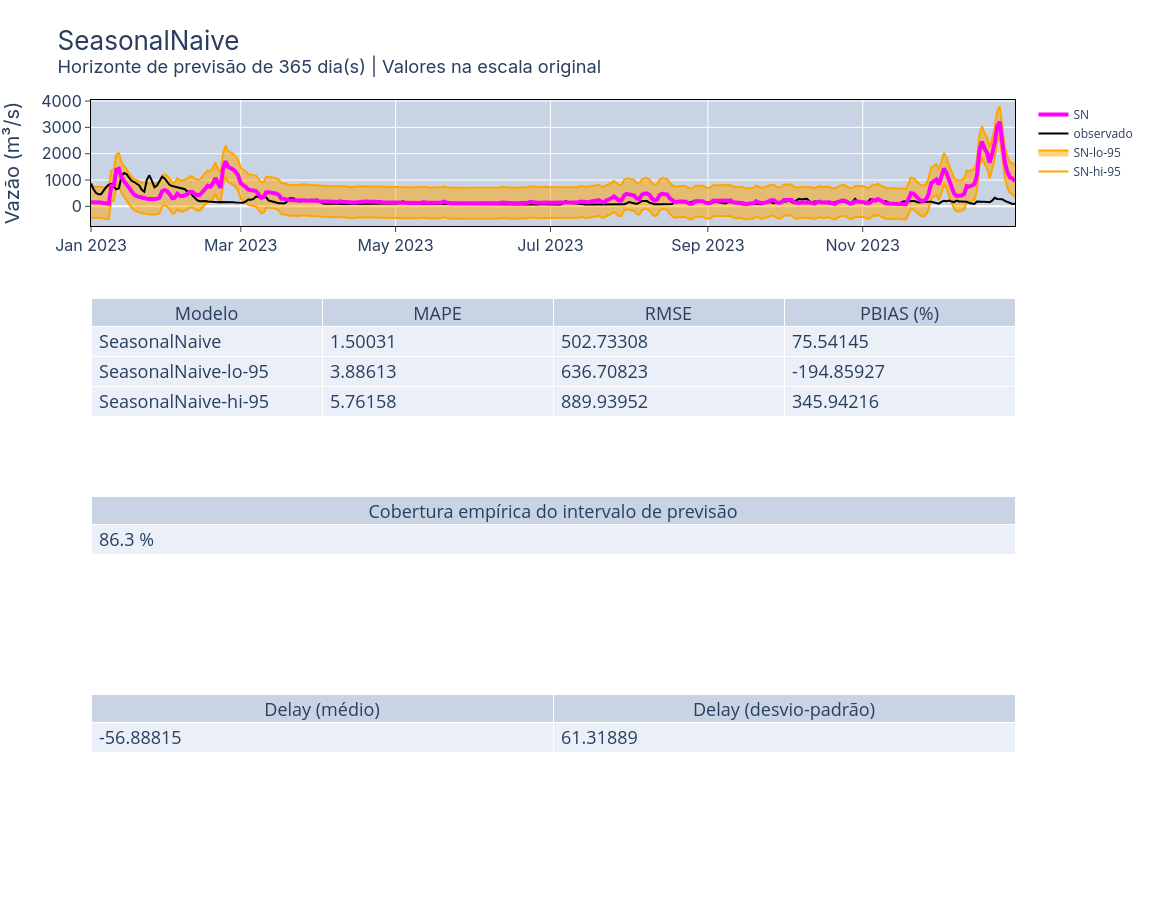
\includegraphics[scale=0.33]{Figuras/jequiti/resultados/SN_WFV.png}
	\caption{Resultado do SeasonalNaive no teste \textit{Walk-Forward Validation}\\(fonte: o autor)}
	\label{fig:jequiti_SN_WFV}
\end{figure}

%\begin{table}[!h]
%	\centering \small
%	\caption{Resultados SeasonalNaive - rio Jequitinhonha \\(fonte: o autor)}
%	\begin{tabular}{|l|r|r|r|r|r|r|} \hline 
	%		\textbf{Horizonte} & \textbf{MAPE} & \textbf{RMSE} & \textbf{PBIAS} \\\hline
	%		1 dia              & 0,871         & 831,44        & -87,11 \\\hline
	%		3 dias             & 1,528         & 1872,25       & 102,71 \\\hline
	%		7 dias             & 1,046         & 1529,13       & 49,64  \\\hline
	%		15 dias            & 0,791         & 1468,02       & -13,46 \\\hline
	%	\end{tabular}
%	\label{tab:sn_jequitinhonha_resultados}
%\end{table}

Os resultados obtidos com o modelo de Regressão Linear apresentaram-se bastante promissores. Nesta fase inicial de avaliação os dados foram log-transformados, conforme indicado no título, que menciona a condição ``destransformados''. A destransformação foi aplicada para garantir que o gráfico estivesse em uma escala mais acessível e interpretável para o leitor. \underline{Esta nomenclatura será mantida ao longo de todo o trabalho}.

Os resultados obtidos utilizando o modelo de Regressão Linear mostraram-se bastante promissores. Nesta primeira avaliação, os dados foram log-transformados. Isso é verificável no título, com o uso de ``(destransformados)''. Os dados foram log-transformados e destransformados para desenhar o gráfico, para ficar numa escala acessível para quem lê. Essa dinâmica no título se manterá por todo trabalho.

Partindo pela KGE calculada, o resultado mostrou-se excelente. Recordando: quanto mais próxima de 1, melhor. Este valor sugere que o modelo é eficaz na previsão do comportamento hidrológico do sistema em análise, oferecendo previsões que estão bem alinhadas com os dados observados. A MAPE de 14\% sugere que o modelo tem uma precisão razoável e é bastante confiável. O modelo apresentou um viés sistemático de subestimar os resultados, conforme aponta a PBIAS de -1,76\%. Considerando todas as métricas, o resultado indica que o modelo teve um desempenho global muito bom. A KGE alta é particularmente indicativa de um bom ajuste global, com o modelo capturando bem tanto a dinâmica quanto a magnitude dos dados observados.

Considerando a qualidade dos intervalos de previsão, a cobertura observada de 97,81\% excedeu o intervalo teórico calculado de 95\%, o que, à primeira vista, poderia ser interpretado como um desempenho satisfatório. No entanto, o limite superior do intervalo (hi-95) mostrou-se excessivamente elevado nos meses de janeiro e fevereiro, o que pode comprometer a interpretação dos resultados. Isso ocorre porque intervalos de previsão excessivamente amplos podem capturar praticamente qualquer valor observado, reduzindo a utilidade prática da previsão.

É importante destacar que os intervalos de previsão são calculados a partir dos erros do modelo durante a etapa de treinamento (\textit{in-sample residuals}). Para uma análise mais aprofundada desse comportamento, é necessário examinar os dados anteriores a 2023. A Figura \ref{fig:jequiti_LR_final_2022_detalhe} revela que, nos últimos dias de 2022, houve observações significativamente elevadas. É provável que os erros associados a esse período mais próximo tenham influenciado a amplitude dos intervalos de previsão subsequentes. Essa interpretação é suportada pela observação de que o comportamento ao final de 2023 foi mais estável, possivelmente devido à ausência de eventos ruidosos imediatamente anteriores.

\begin{figure}[!h]
	\centering
	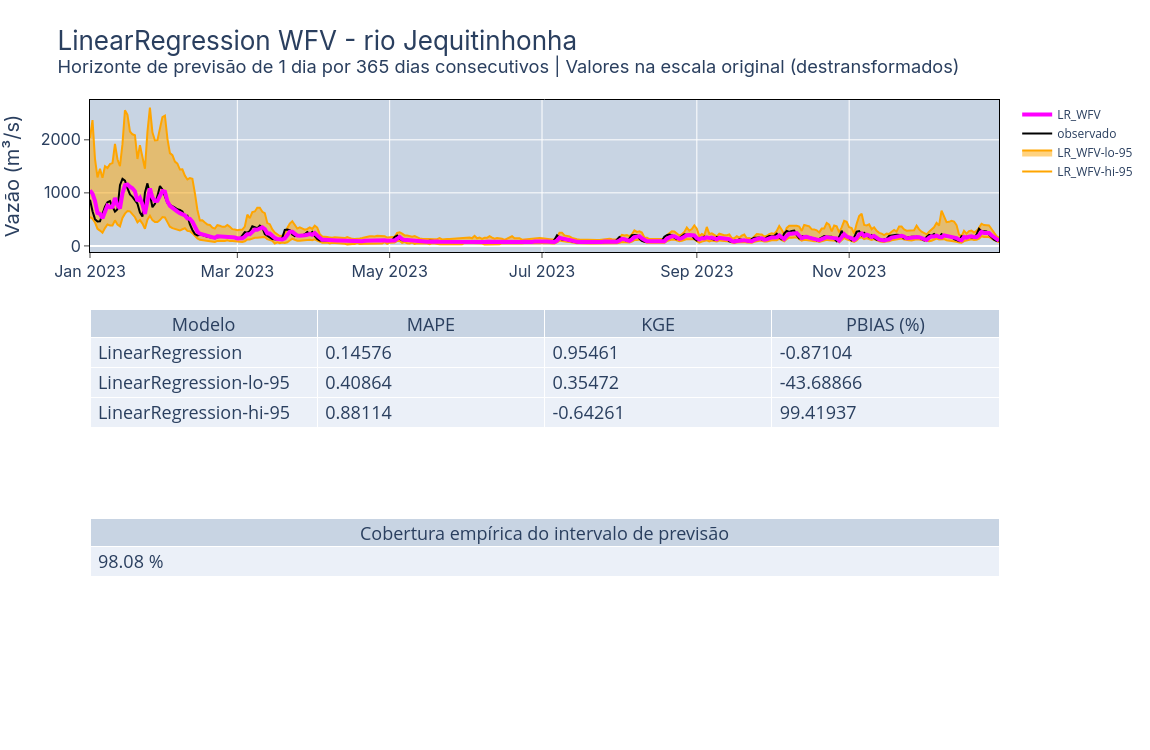
\includegraphics[scale=0.33]{Figuras/jequiti/resultados/LR_WFV_LOG.png}
	\caption{\textit{Walk-Forward Validation} para o modelo Regressão Linear\\(fonte: o autor)}
	\label{fig:jequiti_LR_WFV_LOG}
\end{figure}

\begin{figure}[!h]
	\centering
	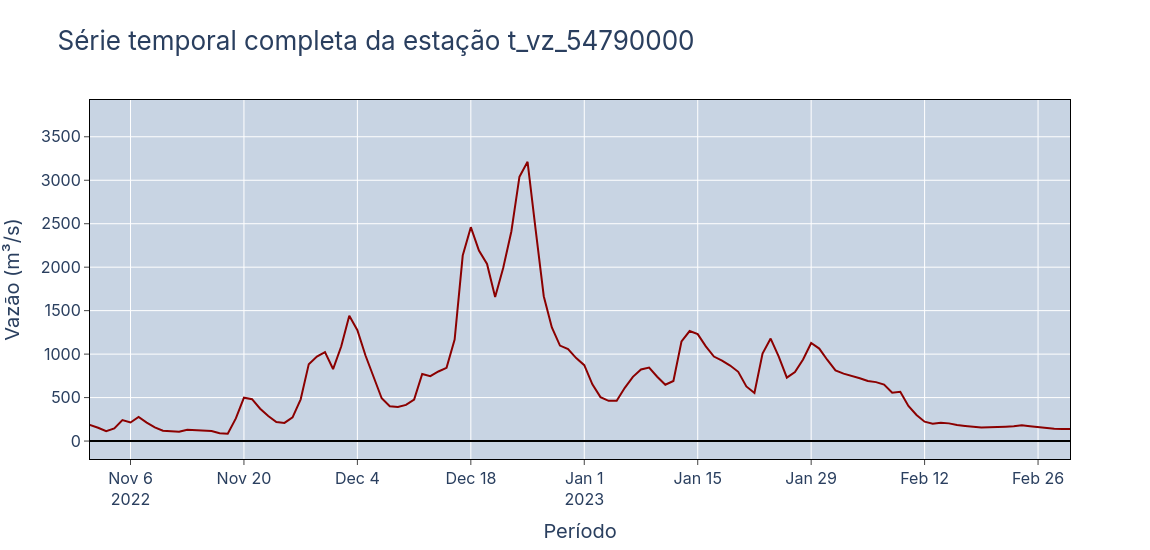
\includegraphics[scale=0.33]{Figuras/jequiti/resultados/LR_final_2022_detalhe.png}
	\caption{Detalhe do trecho final dos dados, em 2022, usados para treinamento.\\(fonte: o autor)}
	\label{fig:jequiti_LR_final_2022_detalhe}
\end{figure}

A análise de delay mostrou um resultado médio de $-0,87$. Considerando que os dados estão numa frequência diária, isso pode ser interpretado como o modelo atrasando a previsão em 0,87 dias, o que seria menos d2 24 horas entre o evento ocorrer e ele ser percebido na previsão. Acredito que afirmar que o modelo está atrasado 20,88 horas não converge com a realidade, por isso que se considerar o desvio-padrão no resultado, confere mais coerência, pois indicaria que o atraso percebido no fenômeno é de cerca de um dia e meio, dois dias. Se pegar a série prevista pelo modelo e comprimir linearmente em -0,87, ambas as sequências serão idênticas, ou seja, a série prevista será a série observada.

\begin{figure}[!h]
	\centering
	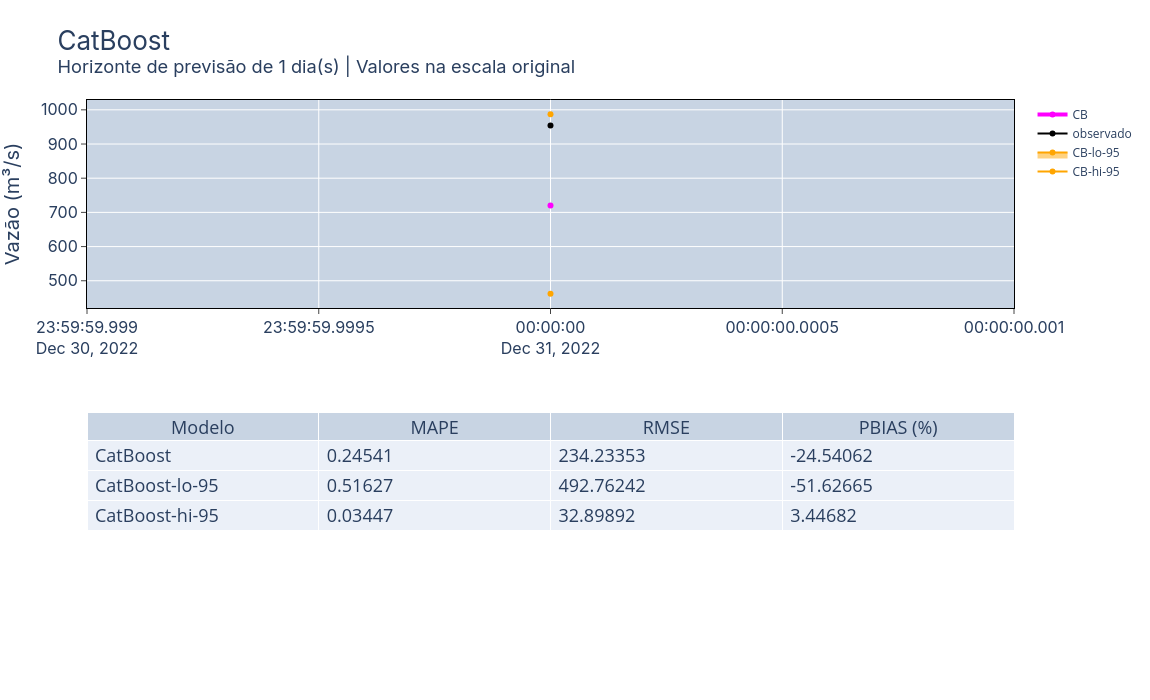
\includegraphics[scale=0.33]{Figuras/jequiti/resultados/CatBoost_fh1.png}
	\caption{CatBoost para o horizonte de previsão de 1 dia\\(fonte: o autor)}
	\label{fig:jequiti_CatBoostRegressor_fh1}
\end{figure}

\begin{figure}[!h]
	\centering
	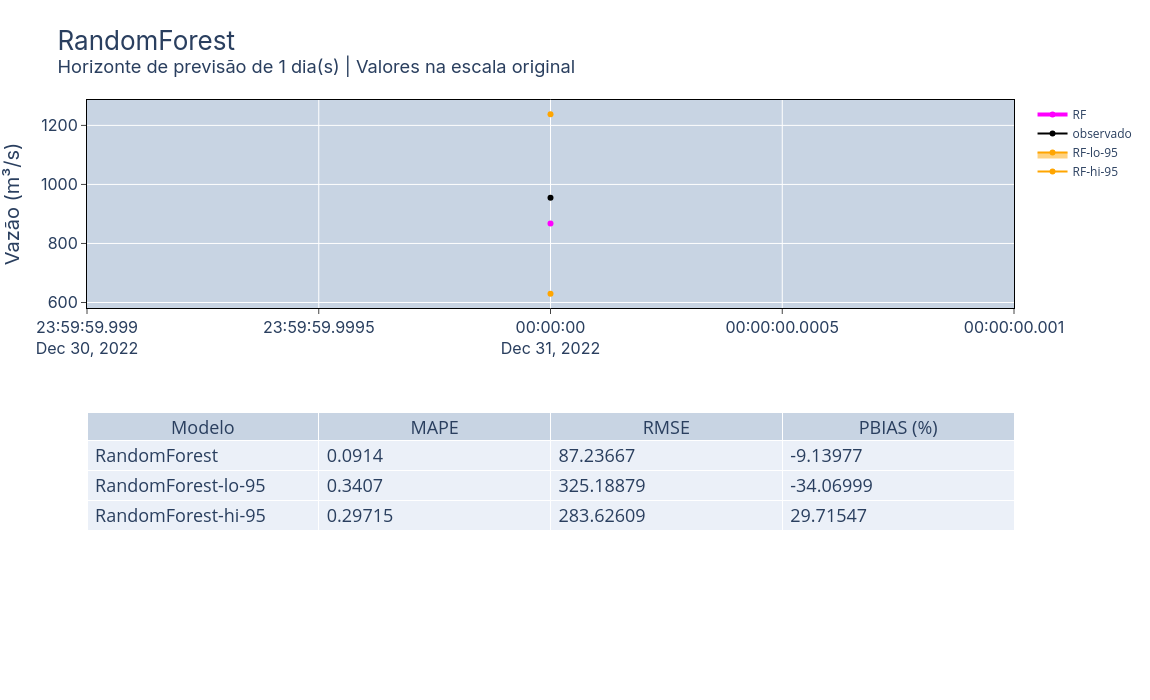
\includegraphics[scale=0.33]{Figuras/jequiti/resultados/RandomForest_fh1.png}
	\caption{RandomForest para o horizonte de previsão de 1 dia\\(fonte: o autor)}
	\label{fig:jequiti_RandomForest_fh1}
\end{figure}

\begin{figure}[!h]
	\centering
	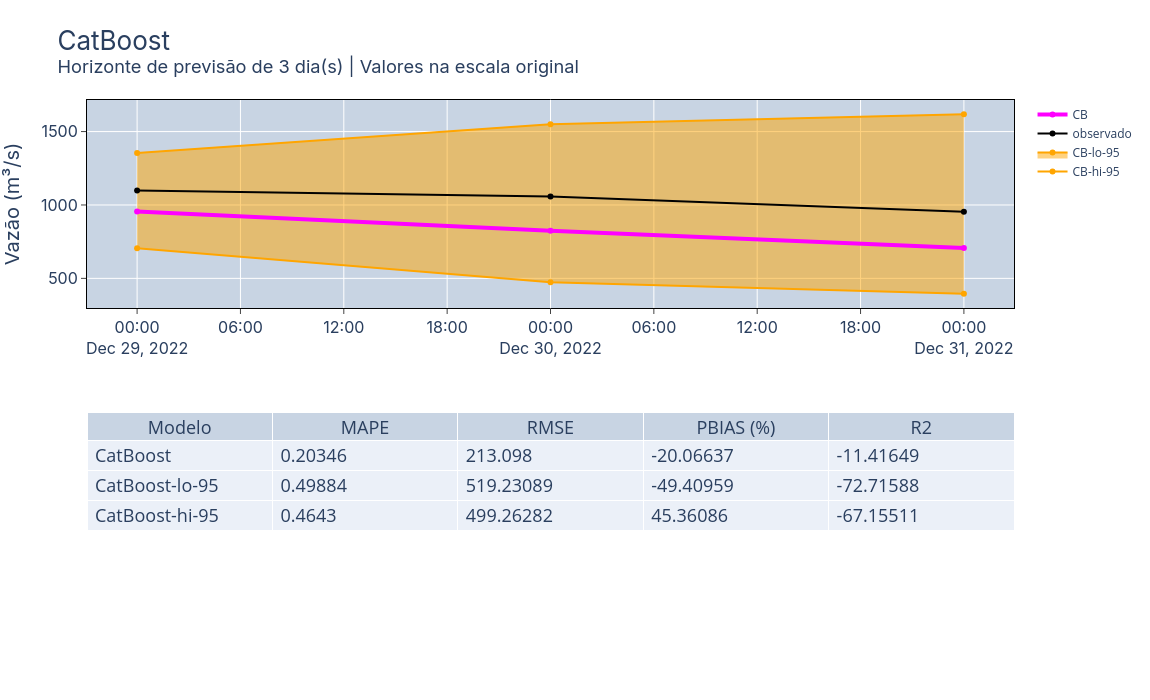
\includegraphics[scale=0.33]{Figuras/jequiti/resultados/CatBoost_fh3.png}
	\caption{CatBoost para o horizonte de previsão de 3 dias\\(fonte: o autor)}
	\label{fig:jequiti_CatBoostRegressor_fh3}
\end{figure}

\begin{figure}[!h]
	\centering
	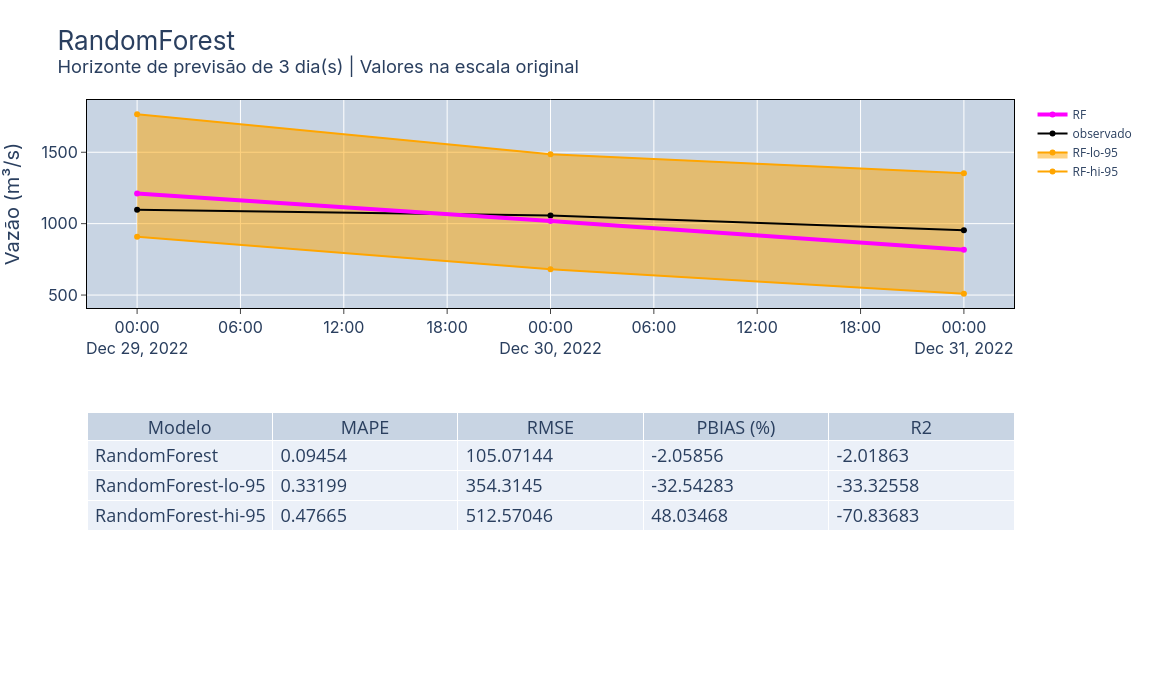
\includegraphics[scale=0.33]{Figuras/jequiti/resultados/RandomForest_fh3.png}
	\caption{RandomForest para o horizonte de previsão de 3 dias\\(fonte: o autor)}
	\label{fig:jequiti_RandomForest_fh3}
\end{figure}

\begin{figure}[!h]
	\centering
	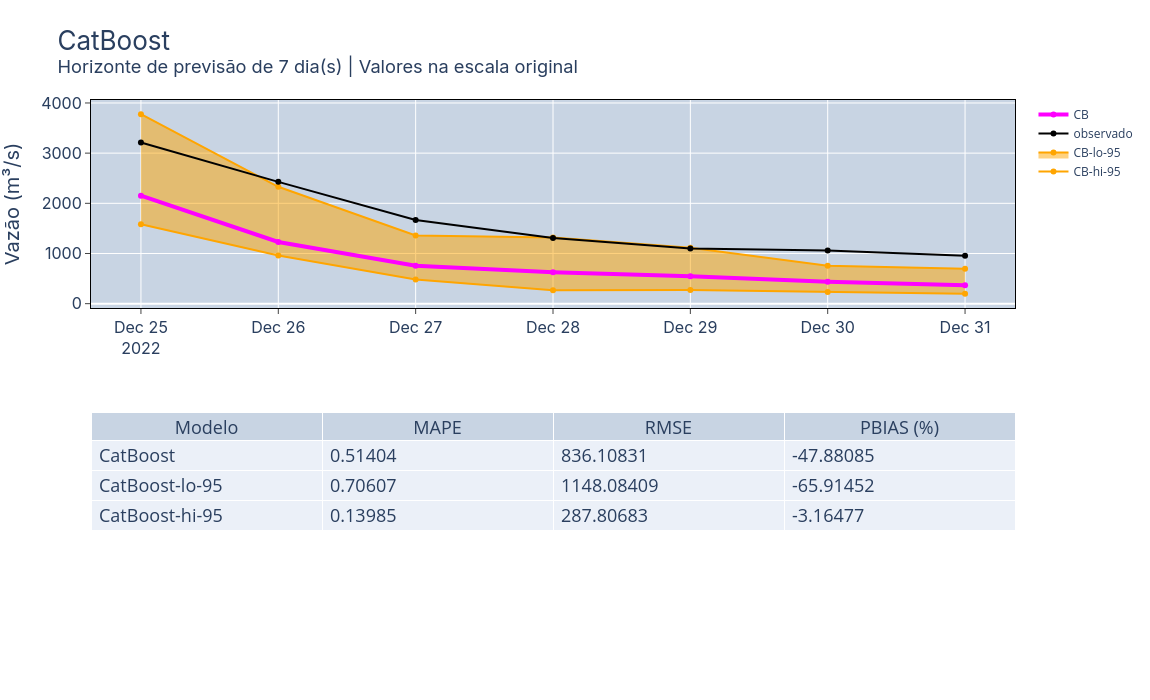
\includegraphics[scale=0.33]{Figuras/jequiti/resultados/CatBoost_fh7.png}
	\caption{CatBoost para o horizonte de previsão de 7 dias\\(fonte: o autor)}
	\label{fig:jequiti_CatBoostRegressor_fh7}
\end{figure}

\begin{figure}[!h]
	\centering
	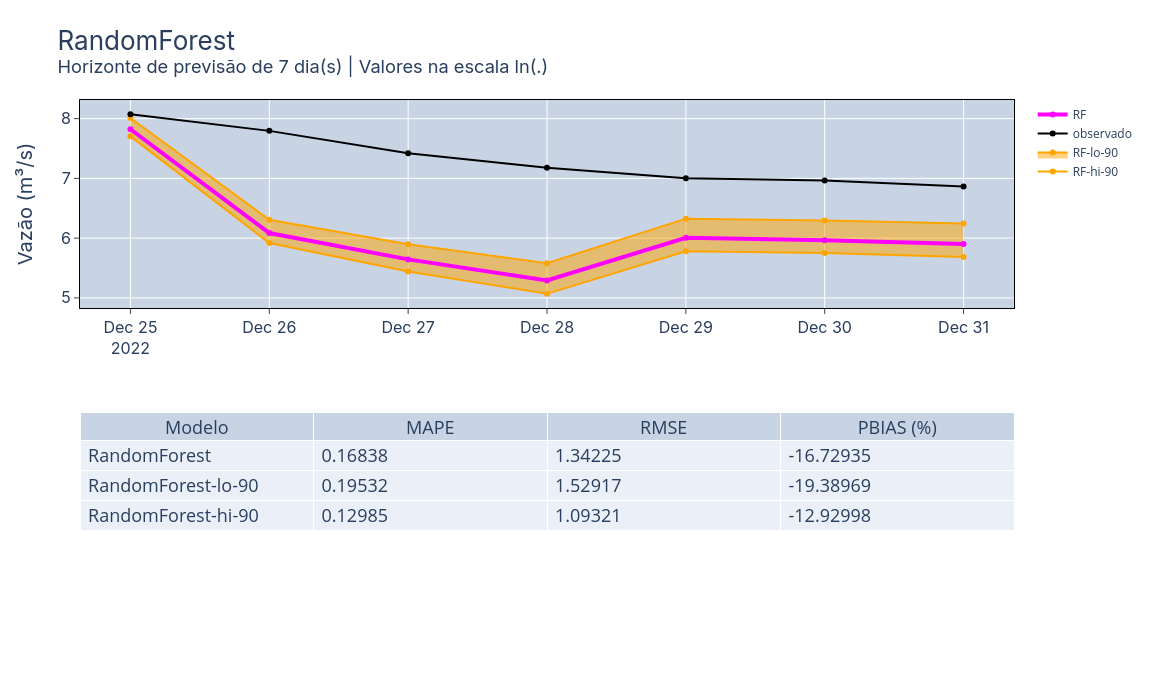
\includegraphics[scale=0.33]{Figuras/jequiti/resultados/RandomForest_fh7.png}
	\caption{RandomForest para o horizonte de previsão de 7 dias\\(fonte: o autor)}
	\label{fig:jequiti_RandomForest_fh7}
\end{figure}

\begin{figure}[!h]
	\centering
	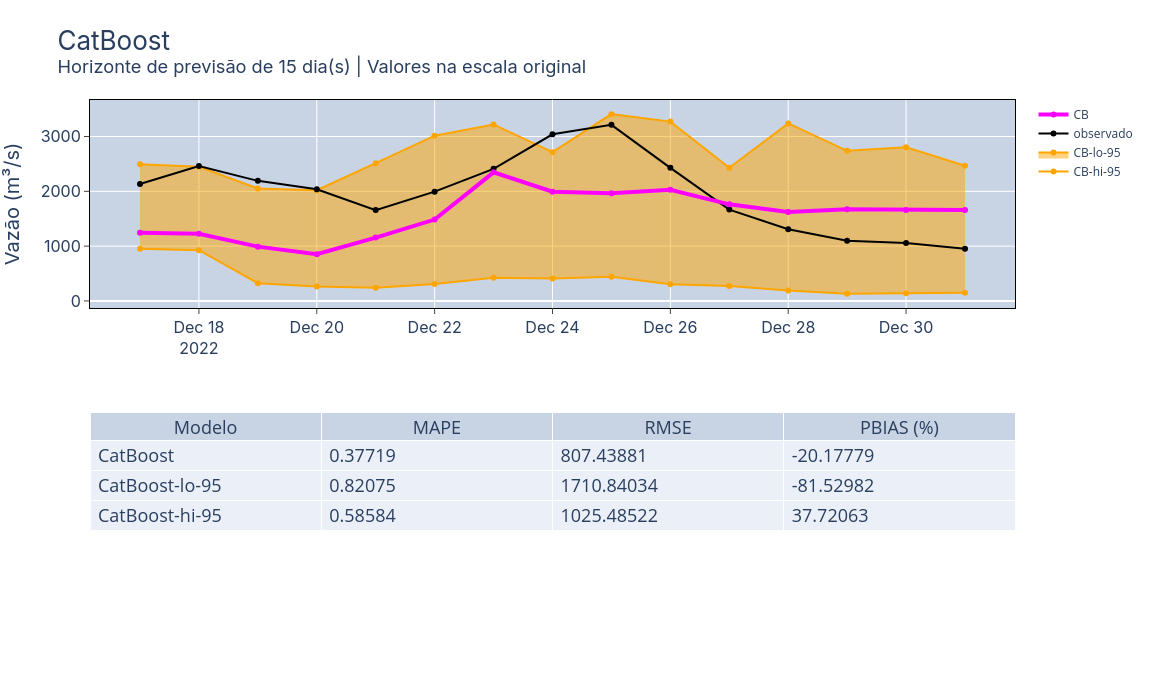
\includegraphics[scale=0.33]{Figuras/jequiti/resultados/CatBoost_fh15.png}
	\caption{CatBoost para o horizonte de previsão de 15 dias\\(fonte: o autor)}
	\label{fig:jequiti_CatBoostRegressor_fh15}
\end{figure}

\begin{figure}[!h]
	\centering
	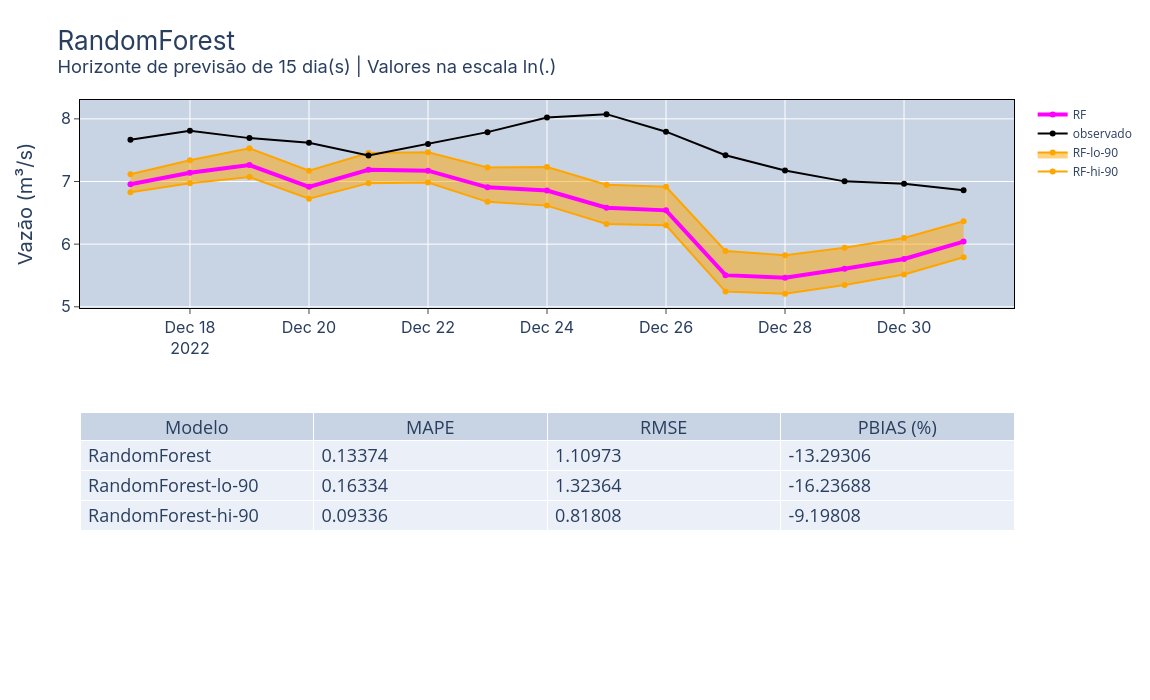
\includegraphics[scale=0.33]{Figuras/jequiti/resultados/RandomForest_fh15.png}
	\caption{RandomForest para o horizonte de previsão de 15 dias\\(fonte: o autor)}
	\label{fig:jequiti_RandomForest_fh15}
\end{figure}
\clearpage

\section{Importância das variáveis}
%Analisar a importância das variáveis contínuas e categóricas na previsão (feature importance).

\section{Discuss\~ao dos resultados}
%Interpretar os resultados e discutir as limitações. Se possível, comparar com estudos anteriores.